\chapter{ह्युकेल सिद्धांत और संयुग्मित निकाय}\label{ch:b2:huckel}

साइक्लोहेक्सीन में हाइड्रोजन मिलाइए तो प्रति मोल \qty{119}{kJ} मुक्त होते हैं। बेन्ज़ीन,
छह कार्बनों के वलय में तीन द्वि-आबंधों के साथ, साइक्लोहेक्सेन तक पहुँचते हुए
तिगुनी ऊर्जा मुक्त करनी चाहिए; वह \qty{150}{kJ} कम मुक्त करती है। वह लुप्त
ऊर्जा \omterm{def:b2:huckel:aromatic}{ऐरोमैटिक} वलय का स्थायित्व है, वही कारण जिससे बेन्ज़ीन
उन योगात्मक अभिक्रियाओं का प्रतिरोध करती है जो ऐल्कीन करते हैं। 1931 में एरिख ह्युकेल ने अणु को
उसके $\pi$ इलेक्ट्रॉनों और उनके पड़ोसियों तक घटाकर इसे एक सारणिक से
परिकलित किया। उनकी विधि स्थूल है, परंतु यह समझाती है कि छह $\pi$
इलेक्ट्रॉनों वाले वलय विशेष क्यों हैं, लंबी संयुग्मित शृंखलाएँ दृश्य प्रकाश क्यों अवशोषित करती हैं, और
संयुग्मित अणु अपने आवेश कहाँ रखता है।

\begin{recall}
\Cref{ch:b2:diatomic-mos}: \omterm{def:b2:diatomic-mos:integrals}{कूलॉम समाकल} $\alpha$, \omterm{def:b2:diatomic-mos:integrals}{अनुनाद समाकल} $\beta$,
\omterm{def:b2:diatomic-mos:integrals}{सेकुलर सारणिक}। \Cref{ch:b2:fragment-orbitals}: एथीन और
ऐलिल के $\pi$ कक्षक। प्रथम वर्ष का खंड: संयुग्मित निकाय, अनुनाद, वर्णमूलक और
अवशोषण अधिकतम।
\end{recall}

\section{ह्युकेल विधि}

समतलीय संयुग्मित अणु में $\sigma$ कक्षक उस तल के सापेक्ष सममित हैं और तल के लंबवत p
कक्षक प्रतिसममित: वे मिश्रित नहीं होते
(\cref{prop:b2:diatomic-mos:symmetry}), और $\pi$ इलेक्ट्रॉनों पर
अलग से विचार किया जा सकता है।

\begin{definition}[ह्युकेल विधि]\label{def:b2:huckel:method}
\emph{ह्युकेल विधि}\index{ह्युकेल विधि} किसी
समतलीय संयुग्मित निकाय के $\pi$ कक्षकों को प्रति परमाणु एक p कक्षक के संयोजनों $\psi = \sum_r c_r p_r$ के रूप में
परिकलित करती है, इन सन्निकटनों के साथ: अतिव्यापन $S_{rs} = 0$, जब $r \neq s$ (और 1 जब $r =
s$); सभी \omterm{def:b2:diatomic-mos:integrals}{कूलॉम समाकल} $\alpha$ के बराबर; \omterm{def:b2:diatomic-mos:integrals}{अनुनाद समाकल} आबंधित पड़ोसियों के बीच
$\beta < 0$ के बराबर और अन्यथा शून्य।
\end{definition}

$x = (\alpha - E)/\beta$ के साथ सेकुलर समीकरण, हर परमाणु $r$ के लिए,
$xc_r + \sum_{s \text{ का पड़ोसी } r} c_s = 0$ बन जाते हैं, और ऊर्जाएँ उस
सारणिक के मूल हैं जिसके विकर्ण पर $x$ और आबंधित परमाणुओं के बीच 1 है। तुल्य रूप से, $E =
\alpha + m\beta$, जहाँ $m$ अणु के कार्बन ढाँचे के आसन्नता आव्यूह के अभिलक्षणिक मान हैं;
चूँकि $\beta < 0$, धनात्मक $m$ एक आबंधी स्तर है।

\begin{method}[ह्युकेल परिकलन]\label{met:b2:huckel:huckel}
\begin{enumerate}
  \item संयुग्मित परमाणुओं को क्रमांकित कीजिए; विकर्ण पर 0 और हर आबंधित
        युग्म के लिए 1 वाला आव्यूह लिखिए।
  \item उसके अभिलक्षणिक मान $m_k$ ज्ञात कीजिए (नीचे के संवृत रूपों से, या संख्यात्मक रूप से): $E_k =
        \alpha + m_k\beta$।
  \item सबसे अधिक आबंधी स्तर से आरंभ करके, हर एक में दो इलेक्ट्रॉन, स्तर भरिए:
        $E_\pi = \sum_k n_k E_k$।
  \item प्रसामान्यीकृत गुणांकों से आवेश और आबंध सूचकांक परिकलित कीजिए।
\end{enumerate}
\end{method}

\begin{proposition}[अनुरेख]\label{prop:b2:huckel:trace}
किसी ह्युकेल निकाय के $n$ $\pi$ कक्षकों की ऊर्जाओं का योग $n\alpha$ होता है।
\end{proposition}

\begin{proof}
किसी आव्यूह के अभिलक्षणिक मानों का योग उसका अनुरेख होता है; ह्युकेल आव्यूह में $\alpha$
उसके $n$ विकर्ण अवयवों में से हर एक पर है।
\end{proof}

\section{रैखिक पॉलिईन}

\begin{theorem}[रैखिक शृंखला के स्तर]\label{thm:b2:huckel:polyene}
$n$ परमाणुओं वाली रैखिक संयुग्मित शृंखला के स्तर और गुणांक ये हैं:
\[
  E_k = \alpha + 2\beta\cos\frac{k\pi}{n + 1}, \qquad
  c_{jk} = \sqrt{\frac{2}{n + 1}}\,\sin\frac{jk\pi}{n + 1}, \qquad k = 1, \dots, n .
\]
\end{theorem}

\begin{proof}
सेकुलर समीकरण $c_{j-1} + xc_j + c_{j+1} = 0$ हैं, $j = 1, \dots, n$ के लिए,
$c_0 = c_{n+1} = 0$ के साथ। $c_j = \sin j\theta$ आज़माइए: $\sin(j - 1)\theta + \sin(j + 1)\theta = 2\sin
j\theta\cos\theta$, अतः समीकरण $x = -2\cos\theta$ के साथ संतुष्ट होते हैं, और $c_0 = 0$
स्वतः। अंत्य शर्त $c_{n+1} = \sin(n + 1)\theta = 0$ से $\theta =
k\pi/(n + 1)$ मिलता है। तब $E = \alpha - x\beta = \alpha + 2\beta\cos\theta$। प्रसामान्यीकरण में
$\sum_{j=1}^n\sin^2 j\theta = (n + 1)/2$ प्रयुक्त होता है।
\end{proof}

\begin{example}[ब्यूटाडाईन]\label{ex:b2:huckel:butadiene}
$n = 4$ के लिए: $E = \alpha \pm 1.618\beta$, $\alpha \pm 0.618\beta$। चार $\pi$ इलेक्ट्रॉन दोनों
आबंधी स्तरों को भरते हैं: $E_\pi = 4\alpha + 2(1.618 + 0.618)\beta = 4\alpha + 4.472\beta$। सबसे निचले
कक्षक के गुणांक 0.372, 0.602, 0.602, 0.372 हैं, अगले के 0.602, 0.372,
$-0.372$, $-0.602$।
\end{example}

\begin{omfigure}
\begin{tikzpicture}[font=\small]
  \foreach \k/\a/\b/\c/\d/\lab in {1/0.372/0.602/0.602/0.372/{$\psi_1$, $\alpha + 1.618\beta$},
      2/0.602/0.372/-0.372/-0.602/{$\psi_2$, $\alpha + 0.618\beta$},
      3/0.602/-0.372/-0.372/0.602/{$\psi_3$, $\alpha - 0.618\beta$},
      4/0.372/-0.602/0.602/-0.372/{$\psi_4$, $\alpha - 1.618\beta$}} {
    \begin{scope}[yshift={(\k-1)*2.1cm}]
      \draw[black!40] (-0.2,0) -- (3.2,0);
      \pic at (0,0) {omp={1.6*\a}{90}}; \pic at (1,0) {omp={1.6*\b}{90}};
      \pic at (2,0) {omp={1.6*\c}{90}}; \pic at (3,0) {omp={1.6*\d}{90}};
      \node[anchor=west] at (3.6,0) {\lab};
    \end{scope}
  }
\end{tikzpicture}

{\small ब्यूटाडाईन के चार $\pi$ कक्षक, पालि ह्युकेल
गुणांकों (परिकलित) के अनुपात में खींचे गए और उनके चिह्न के अनुसार रंगे गए; ऊर्जाएँ ऊपर की ओर
बढ़ती हैं, $0, 1, 2, 3$ नोडों के साथ। निचले दोनों कक्षक भरे हैं।}
\end{omfigure}

\begin{definition}[$\pi$ आवेश और आबंध सूचकांक]\label{def:b2:huckel:indices}
जब $n_k$ इलेक्ट्रॉन (0, 1 या 2) कक्षक $k$ में हों और गुणांक $c_{rk}$ वास्तविक हों, तो
\emph{$\pi$ आवेश}\index{पाई आवेश@$\pi$ आवेश}, परमाणु $r$ पर, $q_r = \sum_k n_kc_{rk}^2$ है (वह जितने
$\pi$ इलेक्ट्रॉन रखता है उनकी संख्या), और \emph{$\pi$ आबंध सूचकांक}\index{पाई आबंध सूचकांक@$\pi$ आबंध सूचकांक},
आबंध $rs$ का, $p_{rs} = \sum_k n_kc_{rk}c_{sk}$ है।
\end{definition}

ब्यूटाडाईन के लिए $p_{12} = 2(0.372 \times 0.602 + 0.602 \times 0.372) = 0.894$ और $p_{23} =
2(0.602^2 - 0.372^2) = 0.447$: सिरे के आबंध अधिकांश $\pi$ आबंधन वहन करते हैं और
छोटे हैं, केंद्रीय आबंध में आंशिक द्वि-आबंध लक्षण है। सभी आवेश
1 हैं।

\begin{proposition}[एकांतरी हाइड्रोकार्बन]\label{prop:b2:huckel:alternant}
ऐसे उदासीन हाइड्रोकार्बन में, जिसके संयुग्मित परमाणुओं को दो समुच्चयों में इस प्रकार रंगा जा सके
कि किसी समुच्चय के दो पड़ोसी न हों (कोई विषम वलय नहीं), हर $\pi$ आवेश 1 के बराबर होता है।
\end{proposition}

\admitted

यह परिणाम (कूल्सन और रशब्रुक) ऊपर ब्यूटाडाईन पर और सममिति द्वारा बेन्ज़ीन पर
जाँचा गया है; यही कारण है कि ऐसे हाइड्रोकार्बनों में उनके
$\pi$ इलेक्ट्रॉनों से कोई स्थायी द्विध्रुव नहीं होता।

\begin{definition}[विस्थानीकरण ऊर्जा]\label{def:b2:huckel:delocalisation}
किसी संयुग्मित निकाय की \emph{विस्थानीकरण ऊर्जा}\index{विस्थानीकरण ऊर्जा}
उसकी $\pi$ ऊर्जा और उतने ही
पृथक द्वि-आबंधों की ऊर्जा का अंतर है, जिनमें से हर एक की $E_\pi = 2\alpha + 2\beta$ है।
\end{definition}

ब्यूटाडाईन के लिए यह $4.472\beta - 4\beta = 0.472\beta$ है; हेक्साट्राईन के लिए $0.988\beta$।

\section{वलय और ऐरोमैटिकता}

\begin{theorem}[वलय के स्तर]\label{thm:b2:huckel:ring}
$n$ संयुग्मित परमाणुओं के समतलीय वलय के स्तर $E_k = \alpha + 2\beta\cos(2\pi k/n)$ हैं,
$k = 0, 1, \dots, n - 1$: एक निम्नतम स्तर $\alpha + 2\beta$, फिर अपभ्रष्ट स्तरों के
युग्म, और सम $n$ के लिए एक उच्चतम स्तर $\alpha - 2\beta$।
\end{theorem}

\begin{proof}
वलय में हर परमाणु के दो पड़ोसी होते हैं, सूचकांक $n$ मापांक में लिए जाते हैं:
$c_{j-1} + xc_j + c_{j+1} = 0$ सभी $j$ के लिए, और $c_{j+n} = c_j$। $c_j = \mathrm e^{\mathrm
i jq}$ आज़माइए: समीकरण $x = -(\mathrm e^{-\mathrm iq} + \mathrm e^{\mathrm iq}) = -2\cos q$ देता है,
और आवर्तिता $nq = 2\pi k$ माँगती है। स्तर $k$ और $n - k$ की ऊर्जा समान
है; उनका योग और अंतर वास्तविक कक्षक हैं। केवल $k = 0$ (और $k = n/2$, सम $n$ के लिए)
अकेला है।
\end{proof}

\begin{corollary}[फ़्रॉस्ट वृत्त]\label{cor:b2:huckel:frost}
किसी वलय के स्तर $2|\beta|$ त्रिज्या के, $\alpha$ पर केंद्रित, वृत्त पर पढ़े जाते हैं, जिसमें
एक सम $n$-भुज इस प्रकार अंतर्निर्मित है कि एक शीर्ष तली पर हो: हर शीर्ष
किसी स्तर की ऊँचाई पर है।
\end{corollary}

\begin{proof}
बहुभुज का शीर्ष $k$ कोण $-\pi/2 + 2\pi k/n$ पर है, केंद्र के सापेक्ष ऊँचाई
$-2|\beta|\cos(2\pi k/n) = 2\beta\cos(2\pi k/n)$ पर।
\end{proof}

\begin{omfigure}
\begin{tikzpicture}[font=\scriptsize]
  \foreach \n/\x/\name/\el in {4/0/{\ce{C4H4}}/4, 5/3.4/{\ce{C5H5-}}/6, 6/6.8/{\ce{C6H6}}/6, 7/10.2/{\ce{C7H7+}}/6} {
    \begin{scope}[xshift=\x cm]
      \draw[black!35] (0,0) circle (1.2);
      \draw[black!60] \foreach \k in {0,...,\the\numexpr\n-1\relax} { ({-90+360*\k/\n}:1.2) -- ({-90+360*(\k+1)/\n}:1.2) };
      \foreach \k in {0,...,\the\numexpr\n-1\relax} {
        \draw[very thick] ({1.2*cos(-90+360*\k/\n)-0.22},{1.2*sin(-90+360*\k/\n)}) -- ({1.2*cos(-90+360*\k/\n)+0.22},{1.2*sin(-90+360*\k/\n)});
      }
      \draw[densely dotted] (-1.5,0) -- (1.5,0);
      \node[font=\small] at (0,-1.75) {\name};
    \end{scope}
  }
  \node[anchor=east] at (-1.5,0) {$\alpha$};
  % electrons: C4H4 (2 + 1 + 1), others filled lowest three
  \foreach \x in {0,3.4,6.8,10.2} {
    \draw[-{Stealth[length=1mm]}, thick] ({\x-0.05},-1.32) -- ({\x-0.05},-1.08);
    \draw[-{Stealth[length=1mm]}, thick] ({\x+0.05},-1.08) -- ({\x+0.05},-1.32);
  }
  % six-electron rings: the lowest degenerate pair is filled
  \foreach \n/\x in {5/3.4, 6/6.8, 7/10.2} {
    \foreach \k in {1, \the\numexpr\n-1\relax} {
      \pgfmathsetmacro\ex{\x + 1.2*cos(-90 + 360*\k/\n)}
      \pgfmathsetmacro\ey{1.2*sin(-90 + 360*\k/\n)}
      \draw[-{Stealth[length=1mm]}, thick] ({\ex-0.05},{\ey-0.12}) -- ({\ex-0.05},{\ey+0.12});
      \draw[-{Stealth[length=1mm]}, thick] ({\ex+0.05},{\ey+0.12}) -- ({\ex+0.05},{\ey-0.12});
    }
  }
  % C4H4: one electron in each of the two nonbonding levels
  \draw[-{Stealth[length=1mm]}, thick] (1.2,-0.12) -- (1.2,0.12);
  \draw[-{Stealth[length=1mm]}, thick] (-1.2,-0.12) -- (-1.2,0.12);
\end{tikzpicture}

{\small फ़्रॉस्ट वृत्त। $2|\beta|$ त्रिज्या के वृत्त में तली पर एक शीर्ष के साथ अंतर्निर्मित
हर बहुभुज के शीर्ष वलय के स्तर देते हैं। छह $\pi$
इलेक्ट्रॉनों के साथ \ce{C5H5-}, \ce{C6H6} और \ce{C7H7+} निम्नतम स्तर और एक अपभ्रष्ट
युग्म भरते हैं: संवृत कोश। साइक्लोब्यूटाडाईन के चार इलेक्ट्रॉन दो इलेक्ट्रॉनों को एक
अपभ्रष्ट अनाबंधी युग्म में छोड़ते हैं (खींचे गए)।}
\end{omfigure}

\begin{definition}[ऐरोमैटिकता]\label{def:b2:huckel:aromatic}
कोई चक्रीय, समतलीय, पूर्णतः संयुग्मित निकाय \emph{ऐरोमैटिक}\index{ऐरोमैटिक} है जब
उसके $\pi$ इलेक्ट्रॉन बड़ी \omterm{def:b2:huckel:delocalisation}{विस्थानीकरण ऊर्जा} के साथ एक संवृत कोश बनाते हैं, और
\emph{प्रति-ऐरोमैटिक}\index{प्रति-ऐरोमैटिक} जब उसके $\pi$ इलेक्ट्रॉन किसी अपभ्रष्ट
युग्म को आधा भरते हैं, जो उसे संगत खुली शृंखला से कम स्थायी बनाता है।
\end{definition}

\begin{theorem}[ह्युकेल नियम]\label{thm:b2:huckel:huckel-rule}
किसी समतलीय एकचक्रीय संयुग्मित निकाय में $\pi$ इलेक्ट्रॉनों का संवृत कोश होता है यदि और केवल
यदि उसमें उनकी संख्या $4N + 2$ हो ($N = 0, 1, 2, \dots$); $4N$ के साथ उसके दो इलेक्ट्रॉन एक
आधे भरे अपभ्रष्ट युग्म में होते हैं। यही \emph{ह्युकेल नियम}\index{ह्युकेल नियम} है।
\end{theorem}

\begin{proof}
\cref{thm:b2:huckel:ring} से नीचे से स्तर एक अकेला स्तर और
फिर अपभ्रष्ट युग्म हैं (भरे भाग के लिए)। संवृत कोश अकेले
स्तर (2 इलेक्ट्रॉन) और युग्मों की एक पूर्ण संख्या $N$ (हर एक में 4 इलेक्ट्रॉन) को भरता है: $4N + 2$।
$4N$ इलेक्ट्रॉनों के साथ अंतिम युग्म में केवल दो होते हैं, उसके हर कक्षक में एक (हुंड का
नियम)।
\end{proof}

\begin{method}[क्या यह ऐरोमैटिक है?]\label{met:b2:huckel:aromaticity}
\begin{enumerate}
  \item क्या निकाय ऐसा वलय है जिसके हर परमाणु पर एक p कक्षक हो (कार्बधनायन
        और कार्बऋणायन केंद्रों और विषम-परमाणुओं के एकाकी युग्मों को गिनकर)?
  \item क्या यह समतलीय हो सकता है?
  \item $\pi$ इलेक्ट्रॉन गिनिए: $4N + 2$ \omterm{def:b2:huckel:aromatic}{ऐरोमैटिक}, $4N$ \omterm{def:b2:huckel:aromatic}{प्रति-ऐरोमैटिक} यदि समतलीय हो।
  \item \omterm{def:b2:huckel:aromatic}{प्रति-ऐरोमैटिक} वलय जब संभव हो, समतलता या संयुग्मन से बचता है
        (साइक्लो-ऑक्टाटेट्राईन टब-आकार का है और पॉलिईन की तरह व्यवहार करता है)।
\end{enumerate}
\end{method}

\begin{example}[बेन्ज़ीन]\label{ex:b2:huckel:benzene}
छह $\pi$ इलेक्ट्रॉन $\alpha + 2\beta$ और युग्म $\alpha + \beta$ को भरते हैं: $E_\pi = 6\alpha + 8\beta$।
तीन पृथक द्वि-आबंध $6\alpha + 6\beta$ देते हैं: \omterm{def:b2:huckel:delocalisation}{विस्थानीकरण ऊर्जा} $2\beta$ है,
छह कार्बनों की खुली शृंखला, हेक्साट्राईन ($0.988\beta$), की लगभग दुगुनी: वलय को
बंद करना उतना ही और मूल्यवान है। सममिति से सभी आबंध सूचकांक बराबर हैं ($p = 2/3$), और छहों
आबंध लंबाइयाँ भी, \qty{139.7}{pm}, जो एथीन (\qty{133.9}{pm}) और एथेन
(\qty{153.6}{pm}) की लंबाइयों के बीच है।
% ledger: geo:C6H6.rCC, geo:C2H4.rCC, geo:C2H6.rCC
\end{example}

\begin{omfigure}
\begin{tikzpicture}[font=\small, y=0.013cm, x=1.0cm]
  \draw[thick] (0,0) -- (10.5,0);
  \node[anchor=north] at (5.2,-8) {साइक्लोहेक्सेन ($\Delta_r H = 0$ संदर्भ)};
  % cyclohexene
  \draw[thick, omDef] (0.6,118.8) -- (1.6,118.8); \draw[->, omDef] (1.1,118.8) -- (1.1,4);
  \node[font=\scriptsize, anchor=south, align=center] at (1.1,120) {साइक्लोहेक्सीन\\ \qty{118.8}{kJ/mol}};
  % diene
  \draw[thick, omDef] (3.6,227.7) -- (4.6,227.7); \draw[->, omDef] (4.1,227.7) -- (4.1,4);
  \draw[thick, black!45, densely dashed] (4.7,237.6) -- (5.6,237.6);
  \node[font=\scriptsize, anchor=south, black!60] at (5.15,240) {$2 \times 118.8$};
  \node[font=\scriptsize, anchor=east, align=right] at (3.5,227.7) {साइक्लोहेक्सा-1,3-डाईन\\ \qty{227.7}{kJ/mol}};
  % benzene
  \draw[thick, omDef] (7.6,206.0) -- (8.6,206.0); \draw[->, omDef] (8.1,206.0) -- (8.1,4);
  \node[font=\scriptsize, anchor=east, align=right] at (7.5,206.0) {बेन्ज़ीन\\ \qty{206.0}{kJ/mol}};
  \draw[thick, black!45, densely dashed] (7.6,356.4) -- (8.6,356.4);
  \node[font=\scriptsize, anchor=south, black!60] at (8.1,358) {$3 \times 118.8 = 356.4$};
  \draw[<->, omThm, thick] (8.9,206) -- (8.9,356.4) node[midway, right, font=\scriptsize] {\qty{150}{kJ/mol}};
\end{tikzpicture}

{\small गैस प्रावस्था में साइक्लोहेक्सेन तक हाइड्रोजनन की एन्थैल्पियाँ, सारणीबद्ध
संभवन एन्थैल्पियों से (स्तंभ, ऊँचाई = मुक्त ऊष्मा)। दो संयुग्मित द्वि-आबंध
एक के दुगुने से \qty{10}{kJ/mol} कम मुक्त करते हैं; बेन्ज़ीन एक के तिगुने से \qty{150}{kJ/mol} कम
मुक्त करती है: यही उसका \omterm{def:b2:huckel:aromatic}{ऐरोमैटिक} स्थायीकरण है।}
% ledger: dfh:C6H6_g, dfh:C6H10_g, dfh:C6H12_g, dfh:C6H8_g
\end{omfigure}

\begin{history}[केकुले का वलय]
\begin{minipage}[t]{0.22\linewidth}
\vspace{0pt}
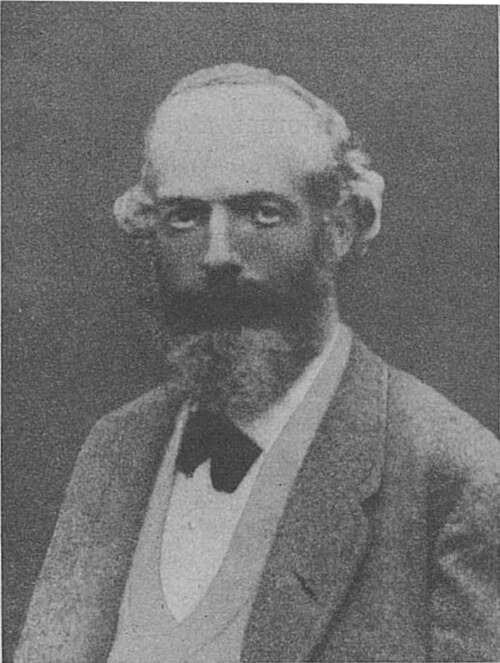
\includegraphics[width=\linewidth]{images/book3/kekule.jpg}
\end{minipage}\hfill
\begin{minipage}[t]{0.74\linewidth}
\vspace{0pt}
1865 में ऑगुस्ट केकुले ने प्रस्तावित किया कि बेन्ज़ीन के छह कार्बन परमाणु
एकांतर एकल और द्वि-आबंधों वाला एक वलय बनाते हैं, और शीघ्र ही यह भी कि दोनों एकांतरण
इतनी तेज़ी से आपस में बदलते हैं कि हर आबंध समान हो जाता है। एक्स-किरण
विवर्तन से मिले समान आबंधों, और पूरे वलय पर फैले $\pi$ कक्षकों ने उनकी अंतर्दृष्टि को
आधुनिक रूप दिया; 1931 में \omterm{thm:b2:huckel:huckel-rule}{ह्युकेल नियम} ने समझाया कि चार या आठ नहीं, बल्कि छह इलेक्ट्रॉन
किसी वलय को विशेष क्यों बनाते हैं। (चित्र, 1873, अज्ञात लेखक, सार्वजनिक अधिकार-क्षेत्र,
विकिमीडिया कॉमन्स।)
\end{minipage}
\end{history}

\section{संयुग्मन और प्रकाश}

\begin{proposition}[पॉलिईन का अंतराल]\label{prop:b2:huckel:gap}
$n$ कार्बनों ($n$ सम) वाले रैखिक पॉलिईन में उच्चतम भरे
और निम्नतम खाली $\pi$ स्तर के बीच का अंतराल $4|\beta|\sin(\pi/(2(n + 1)))$ है: शृंखला
लंबी होने पर यह घटता है।
\end{proposition}

\begin{proof}
उच्चतम भरा स्तर $k = n/2$ है, निम्नतम खाली $k = n/2 + 1$। $\theta_k =
k\pi/(n + 1)$ के साथ, $E_{n/2+1} - E_{n/2} = 2|\beta|(\cos\theta_{n/2} - \cos\theta_{n/2+1}) = 4|\beta|
\sin\frac{\theta_{n/2} + \theta_{n/2+1}}{2}\sin\frac{\theta_{n/2+1} - \theta_{n/2}}{2}$, और
पहली ज्या $\sin(\pi/2) = 1$ है। यह $n$ के साथ घटता है क्योंकि $\sin$,
$[0, \pi/2]$ पर बढ़ता है।
\end{proof}

\begin{omfigure}
\begin{tikzpicture}
\begin{axis}[width=0.5\linewidth, height=5cm, xmin=0, xmax=22, ymin=0, ymax=2.2,
  axis x line=bottom, axis y line=left, xlabel={कार्बन $n$}, ylabel={अंतराल$/|\beta|$},
  tick label style={font=\small}, label style={font=\small}]
\addplot[omThm, thick, mark=*, mark size=1.3pt] table[x=n, y=gap] {figdata/out/bachelor-2-huckel-b.dat};
\end{axis}
\end{tikzpicture}\hfill
\begin{tikzpicture}
\begin{axis}[width=0.48\linewidth, height=5.4cm, xmin=-1, xmax=11, ymin=-2.4, ymax=2.4,
  axis x line=none, axis y line=left, ylabel={$(E - \alpha)/|\beta|$}, clip=false,
  tick label style={font=\small}, label style={font=\small}]
\addplot[only marks, mark=-, mark size=5pt, very thick, omDef] table[x=x, y=e] {figdata/out/bachelor-2-huckel-a.dat};
\draw[densely dotted] (axis cs:-1,0) -- (axis cs:11,0);
\node[anchor=north, font=\scriptsize] at (axis cs:0,-2.45) {C$_2$};
\node[anchor=north, font=\scriptsize] at (axis cs:2,-2.45) {C$_3$};
\node[anchor=north, font=\scriptsize] at (axis cs:4,-2.45) {C$_4$};
\node[anchor=north, font=\scriptsize] at (axis cs:6,-2.45) {C$_6$};
\node[anchor=north, font=\scriptsize] at (axis cs:8,-2.45) {वलय 4};
\node[anchor=north, font=\scriptsize] at (axis cs:10,-2.45) {वलय 6};
\end{axis}
\end{tikzpicture}

{\small बाएँ: रैखिक पॉलिईनों का ह्युकेल अंतराल शृंखला बढ़ने पर घटता है,
यही कारण है कि लंबी संयुग्मित शृंखलाएँ दीर्घतर तरंगदैर्घ्यों पर, दृश्य तक, अवशोषण करती हैं।
दाएँ: एथीन, ऐलिल, ब्यूटाडाईन, हेक्साट्राईन (शृंखलाएँ) और
साइक्लोब्यूटाडाईन तथा बेन्ज़ीन (वलय) के परिकलित स्तर; आबंधी स्तर $\alpha$ से नीचे।}
\end{omfigure}

कोई विषम-परमाणु उसका \omterm{def:b2:diatomic-mos:integrals}{कूलॉम समाकल}, $\alpha_X = \alpha + h\beta$, और उसके आबंधों के
\omterm{def:b2:diatomic-mos:integrals}{अनुनाद समाकल} बदलकर लाया जाता है: समायोज्य प्राचलों वाला एक मॉडल, जो
गुणात्मक परिणाम बनाए रखता है (विद्युत-ऋणात्मक परमाणु, $h > 0$, $\pi$ घनत्व को अपनी ओर
खींचता है), परंतु जिसकी संख्याएँ समंजित होती हैं, व्युत्पन्न नहीं।

\section{अभ्यास}

\begin{exercise}[$\star$]\label{exo:b2:huckel:1}
ऐलिल धनायन, मूलक और ऋणायन के लिए $E_\pi$ दीजिए।
\end{exercise}

\begin{exercise}[$\star$]\label{exo:b2:huckel:2}
ब्यूटाडाईन का $E_\pi$ स्तरों $\alpha \pm 1.618\beta$, $\alpha \pm 0.618\beta$ से परिकलित कीजिए।
\end{exercise}

\begin{exercise}[$\star$]\label{exo:b2:huckel:3}
\omterm{def:b2:huckel:aromatic}{ऐरोमैटिक}, \omterm{def:b2:huckel:aromatic}{प्रति-ऐरोमैटिक} या कोई नहीं (यदि समतलीय हों): बेन्ज़ीन, साइक्लोपेंटाडाईनिल ऋणायन,
साइक्लोपेंटाडाईनिल धनायन, ट्रोपिलियम धनायन \ce{C7H7+}, साइक्लोब्यूटाडाईन, समतलीय
साइक्लो-ऑक्टाटेट्राईन।
\end{exercise}

\begin{exercise}[$\star$]\label{exo:b2:huckel:4}
समतलीय साइक्लो-ऑक्टाटेट्राईन का फ़्रॉस्ट वृत्त खींचिए और उसके आठ $\pi$ इलेक्ट्रॉन रखिए।
\end{exercise}

\begin{exercise}[$\star\star$]\label{exo:b2:huckel:5}
ब्यूटाडाईन की \omterm{def:b2:huckel:delocalisation}{विस्थानीकरण ऊर्जा} परिकलित कीजिए और उसे
$|\beta| = \qty{75}{kJ/mol}$ के साथ \unit{kJ/mol} में दीजिए। साइक्लोहेक्सा-1,3-डाईन के हाइड्रोजनन
आँकड़ों के \qty{10}{kJ/mol} से तुलना कीजिए।
\end{exercise}

\begin{exercise}[$\star\star$]\label{exo:b2:huckel:6}
ब्यूटाडाईन के $\pi$ आबंध सूचकांक परिकलित कीजिए और पूर्वानुमान कीजिए कि उसका कौन-सा C--C आबंध
सबसे छोटा है।
\end{exercise}

\begin{exercise}[$\star\star$]\label{exo:b2:huckel:7}
पंचसदस्यी वलय के स्तर $\alpha + 2\beta$, $\alpha + 0.618\beta$ (दो बार),
$\alpha - 1.618\beta$ (दो बार) हैं। साइक्लोपेंटाडाईनिल ऋणायन और धनायन के लिए उन्हें भरिए और
तुलना कीजिए।
\end{exercise}

\begin{exercise}[$\star\star$]\label{exo:b2:huckel:8}
सप्तसदस्यी वलय के स्तरों से समझाइए कि साइक्लोहेप्टाट्राईनिल ब्रोमाइड
एक लवण, ट्रोपिलियम ब्रोमाइड, की तरह व्यवहार क्यों करता है।
\end{exercise}

\begin{exercise}[$\star\star$]\label{exo:b2:huckel:9}
हेक्साट्राईन पर अनुरेख नियम की जाँच कीजिए, जिसके स्तर $\alpha \pm 1.802\beta$, $\alpha \pm
1.247\beta$, $\alpha \pm 0.445\beta$ हैं।
\end{exercise}

\begin{exercise}[$\star\star\star$]\label{exo:b2:huckel:10}
संवृत रूप से हेक्साट्राईन के स्तर व्युत्पन्न कीजिए, और उसकी \omterm{def:b2:huckel:delocalisation}{विस्थानीकरण ऊर्जा}।
\end{exercise}

\begin{exercise}[$\star\star\star$]\label{exo:b2:huckel:11}
वर्गाकार साइक्लोब्यूटाडाईन में दो अयुग्मित इलेक्ट्रॉन होते। समझाइए कि वास्तविक अणु
आयताकार क्यों है, दो छोटे और दो लंबे आबंधों के साथ।
\end{exercise}

\begin{exercise}[$\star\star\star$]\label{exo:b2:huckel:12}
दो-परमाणु $\pi$ निकाय \ce{C=X} में, $\alpha_X = \alpha + \beta$ (मॉडल मान, $h = 1$) और
$\beta_{\ce{CX}} = \beta$ के साथ, दोनों स्तर और दो इलेक्ट्रॉनों के लिए C तथा X पर $\pi$ आवेश
ज्ञात कीजिए।
\end{exercise}

\section{समस्या: बेन्ज़ीन की लुप्त ऊर्जा}

\begin{problem}[{सप्ताहांत समस्या --- हाइड्रोजनन की एन्थैल्पियों से बेन्ज़ीन का
ऐरोमैटिक स्थायीकरण, बेन्ज़ीन के ह्युकेल स्तर और उसकी विस्थानीकरण
ऊर्जा, $|\beta|$ का मान, और हेक्साट्राईन तथा
साइक्लो-ऑक्टाटेट्राईन से तुलना}]
\label{pb:b2:huckel:1}
आँकड़े: गैसों की संभवन एन्थैल्पियाँ (\unit{kJ/mol}): बेन्ज़ीन 82.9,
साइक्लोहेक्सा-1,3-डाईन 104.6, साइक्लोहेक्सीन $-4.3$, साइक्लोहेक्सेन $-123.1$। आबंध लंबाइयाँ
(pm): बेन्ज़ीन 139.7, एथीन 133.9, एथेन 153.6।
% ledger: dfh:C6H6_g, dfh:C6H8_g, dfh:C6H10_g, dfh:C6H12_g, geo:C6H6.rCC, geo:C2H4.rCC, geo:C2H6.rCC

\medskip
\noindent\textbf{भाग I --- हाइड्रोजनन।}
\begin{enumerate}
  \item साइक्लोहेक्सीन के साइक्लोहेक्सेन में हाइड्रोजनन का $\Delta_r H^\circ$ परिकलित कीजिए।
  \item साइक्लोहेक्सा-1,3-डाईन के लिए यही।
  \item बेन्ज़ीन के लिए यही।
  \item तीन स्वतंत्र द्वि-आबंध कितनी ऊर्जा मुक्त करते?
  \item बेन्ज़ीन का स्थायीकरण निकालिए।
  \item संयुग्मित डाईन के स्थायीकरण से तुलना कीजिए, और टिप्पणी कीजिए।
\end{enumerate}

\medskip
\noindent\textbf{भाग II --- ह्युकेल बेन्ज़ीन।}
\begin{enumerate}[resume]
  \item बेन्ज़ीन का ह्युकेल आव्यूह लिखिए।
  \item वलय सूत्र से उसके स्तर दीजिए।
  \item उन्हें छह $\pi$ इलेक्ट्रॉनों से भरिए।
  \item $E_\pi$ परिकलित कीजिए।
  \item तीन पृथक द्वि-आबंधों का $E_\pi$ परिकलित कीजिए।
  \item \omterm{def:b2:huckel:delocalisation}{विस्थानीकरण ऊर्जा} निकालिए।
  \item अनुरेख नियम की जाँच कीजिए।
\end{enumerate}

\medskip
\noindent\textbf{भाग III --- $|\beta|$ का मान।}
\begin{enumerate}[resume]
  \item \omterm{def:b2:huckel:delocalisation}{विस्थानीकरण ऊर्जा} को भाग I के स्थायीकरण के बराबर रखिए और
        $|\beta|$ ज्ञात कीजिए।
  \item उस मान से ब्यूटाडाईन की \omterm{def:b2:huckel:delocalisation}{विस्थानीकरण ऊर्जा} का पूर्वानुमान कीजिए, और
        भाग I से तुलना कीजिए।
  \item बेन्ज़ीन के $\pi$ आबंध सूचकांक परिकलित कीजिए।
  \item उनकी तुलना ब्यूटाडाईन के सूचकांकों से कीजिए।
  \item समझाइए कि बेन्ज़ीन की आबंध लंबाइयाँ बराबर क्यों हैं और वे कहाँ पड़ती हैं।
\end{enumerate}

\medskip
\noindent\textbf{भाग IV --- अन्य वलय और शृंखलाएँ।}
\begin{enumerate}[resume]
  \item हेक्साट्राईन की \omterm{def:b2:huckel:delocalisation}{विस्थानीकरण ऊर्जा} परिकलित कीजिए और बेन्ज़ीन से तुलना कीजिए।
  \item समतलीय साइक्लो-ऑक्टाटेट्राईन के स्तर दीजिए।
  \item उन्हें आठ इलेक्ट्रॉनों से भरिए: क्या गड़बड़ है?
  \item वास्तविक अणु इससे कैसे बचता है?
  \item साइक्लोब्यूटाडाईन की स्थिति क्या है?
  \item \omterm{thm:b2:huckel:huckel-rule}{ह्युकेल नियम} बताइए।
  \item बेन्ज़ीन की \omterm{def:b2:huckel:delocalisation}{विस्थानीकरण ऊर्जा} को उसके मापे गए स्थायीकरण के बराबर रखकर
        प्राप्त $|\beta|$ का मान बताइए।
\end{enumerate}
\end{problem}
